\let\negmedspace\undefined
\let\negthickspace\undefined
\documentclass[journal,12pt,onecolumn]{IEEEtran}
\usepackage{gvv-book}
\usepackage{gvv}
\usepackage{mathtools}
\usepackage{amssymb,amsfonts,amsthm}
\usepackage{siunitx}
\usepackage{algorithmic}
\usepackage{graphicx}
\graphicspath{{./figs/}}
\usepackage{textcomp}
\usepackage{xcolor}
\usepackage{txfonts}
\usepackage{listings}
\usepackage{enumitem}
\usepackage{gensymb}
\usepackage{comment}
\usepackage{caption}
\usepackage{tkz-euclide}
\usepackage[latin1]{inputenc}
\usepackage{color}
\usepackage{array}
\usepackage{longtable}
\usepackage{calc}
\usepackage{multirow}
\usepackage{multicol}
\usepackage{hhline}
\usepackage{ifthen}
\usepackage{lscape}
\usepackage{tabularx}
\usepackage{float}
\usepackage[breaklinks=true]{hyperref}
\usepackage{cite}


\begin{document}

\title{
ASSIGNMENT 2: GATE PHYSICS \\
IN: INSTRUMENTATION ENGINEERING}
\author{AI25BTECH11006 - Nikhila }
\maketitle


\vspace{2em} 

\begin{center}
\textbf{Q.1-Q.25 carry one mark each.}   
\end{center}


\begin{enumerate}
\item Two matrices $A$ and $B$ are said to be similar if $B = P^{-1} A P$ for some invertible matrix $P$. Which of the following statements is \textbf{NOT TRUE}?

\hfill{\brak{\text{GATE IN 2011}}}

\begin{multicols}{2}
\begin{enumerate}
    \item $\det A = \det B$
    \item Trace of $A$ = Trace of $B$
    \item $A$ and $B$ have the same eigenvectors
    \item $A$ and $B$ have the same eigenvalues
\end{enumerate}
\end{multicols}

\item If a force $\vec{F}$ is derivable from a potential function $V(r)$ where $r$ is the distance from the origin of the coordinate system, it follows that

\hfill{\brak{\text{GATE IN 2011}}}

\begin{multicols}{4}
\begin{enumerate}
    \item $\vec{\nabla} \cdot \vec{F} = 0$
    \item $\overline{\nabla} \cdot \overline{F} = 0$
    \item $\vec{\nabla} V = 0$
    \item $\nabla^{2} V = 0$
\end{enumerate}
\end{multicols}

\item The quantum mechanical operator for the momentum of a particle moving in one dimension is given by

\hfill{\brak{\text{GATE IN 2011}}}

\begin{multicols}{4}
\begin{enumerate}
    \item $i\hbar \dfrac{d}{dx}$
    \item $-i\hbar \dfrac{d}{dx}$
    \item $\dagger \dfrac{\partial}{\partial t}$
    \item $-\dfrac{\hbar^{2}}{2m} \dfrac{d^{2}}{dx^{2}}$
\end{enumerate}
\end{multicols}

\item A Carnot cycle operates on a working substance between two reservoirs at temperatures $T_{1}$ and $T_{2}$ with $T_{1} > T_{2}$. During each cycle, an amount of heat $Q_{1}$ is extracted from the reservoir at $T_{1}$ and an amount $Q_{2}$ is delivered to the reservoir at $T_{2}$. Which of the following statements is \textbf{INCORRECT}?

\hfill{\brak{\text{GATE IN 2011}}}


\begin{enumerate}
    \item Work done in one cycle is $Q_{1} - Q_{2}$
    \item $\dfrac{Q_{1}}{T_{1}} = \dfrac{Q_{2}}{T_{2}}$
    \item Entropy of the hotter reservoir decreases
    \item Entropy of the universe (consisting of the working substance and the two reservoirs) increases
\end{enumerate}


\item In a first order phase transition, at the transition temperature, specific heat of the system

\hfill{\brak{\text{GATE IN 2011}}}

\begin{enumerate}
    \item Diverges and its entropy remains the same
    \item Diverges and its entropy has finite discontinuity
    \item Remains unchanged and its entropy has finite discontinuity
    \item Has finite discontinuity and its entropy diverges
\end{enumerate}

\newpage

\item The semi-empirical mass formula for the binding energy of a nucleus contains a surface correction term. This term depends on the mass number $A$ of the nucleus as

\hfill{\brak{\text{GATE IN 2011}}}

\begin{multicols}{4}
\begin{enumerate}
    \item $A^{-1/3}$
    \item $A^{1/3}$
    \item $A^{2/3}$
    \item $A$
\end{enumerate}
\end{multicols}

\item The population inversion in a two-level laser material \textbf{cannot} be achieved by optical pumping because

\hfill{\brak{\text{GATE IN 2011}}}


\begin{enumerate}
    \item the rate of upward transitions is equal to the rate of downward transitions
    \item the upward transitions are forbidden but downward transitions are allowed
    \item the upward transitions are allowed but downward transitions are forbidden
    \item the spontaneous decay rate of the higher level is very low
\end{enumerate}


\item The temperature $(T)$ dependence of magnetic susceptibility $(\chi)$ of a ferromagnetic substance with a Curie temperature $(T_{c})$ is given by

\hfill{\brak{\text{GATE IN 2011}}}

\begin{multicols}{2}
\begin{enumerate}
    \item for $T < T_{c}$, $\dfrac{C}{T - T_{c}}$
    \item $\dfrac{C}{T - T_{c}}$, $T > T_{c}$
    \item $\dfrac{C}{T \, T_{c}}$ for $T > T_{c}$
    \item for all temperatures $\dfrac{C}{T + T_{c}}$
\end{enumerate}
\end{multicols}
where $C$ is a constant.

\item The order of magnitude of the energy gap of a typical superconductor is

\hfill{\brak{\text{GATE IN 2011}}}

\begin{multicols}{2}
\begin{enumerate}
    \item $1 \ \mathrm{MeV}$
    \item $1 \ \mathrm{keV}$
    \item $1 \ \mathrm{eV}$
    \item $1 \ \mathrm{meV}$
\end{enumerate}
\end{multicols}

\item Which of the following statements is \textbf{CORRECT} for a common emitter amplifier circuit?

\hfill{\brak{\text{GATE IN 2011}}}


\begin{enumerate}
    \item The output is taken from the emitter
    \item There is $180^\circ$ phase shift between input and output voltages
    \item There is no phase shift between input and output voltages
    \item Both $p$-$n$ junctions are forward biased
\end{enumerate}


\item A $3 \times 3$ matrix has elements such that its trace is $11$ and its determinant is $36$. The eigenvalues of the matrix are all known to be positive integers. The largest eigenvalue of the matrix is

\hfill{\brak{\text{GATE IN 2011}}}

\begin{multicols}{4}
\begin{enumerate}
    \item $18$
    \item $12$
    \item $9$
    \item $6$
\end{enumerate}
\end{multicols}

\item A heavy symmetrical top is rotating about its own axis of symmetry (the $z$-axis). If $I_{1}$, $I_{2}$ and $I_{3}$ are the principal moments of inertia along $x$, $y$ and $z$ axes respectively, then

\hfill{\brak{\text{GATE IN 2011}}}

\begin{multicols}{4}
\begin{enumerate}
    \item $I_{2} = I_{3}, \ I_{1} \neq I_{2}$
    \item $I_{1} = I_{y}, \ I_{1} \neq I_{2}$
    \item $I_{1} = I_{2}, \ I_{1} \neq I_{3}$
    \item $I_{1} = I_{2} \neq I_{3}$
\end{enumerate}
\end{multicols}


\newpage

\item An electron with energy E is incident from left on a potential barrier,given by as shown in the figure. 


\begin{center}
    V\brak{x} = 0  for $x < 0$\\
    = $V_0$ for $x > 0$
\end{center}


\begin{figure}[ht!]
    \centering
    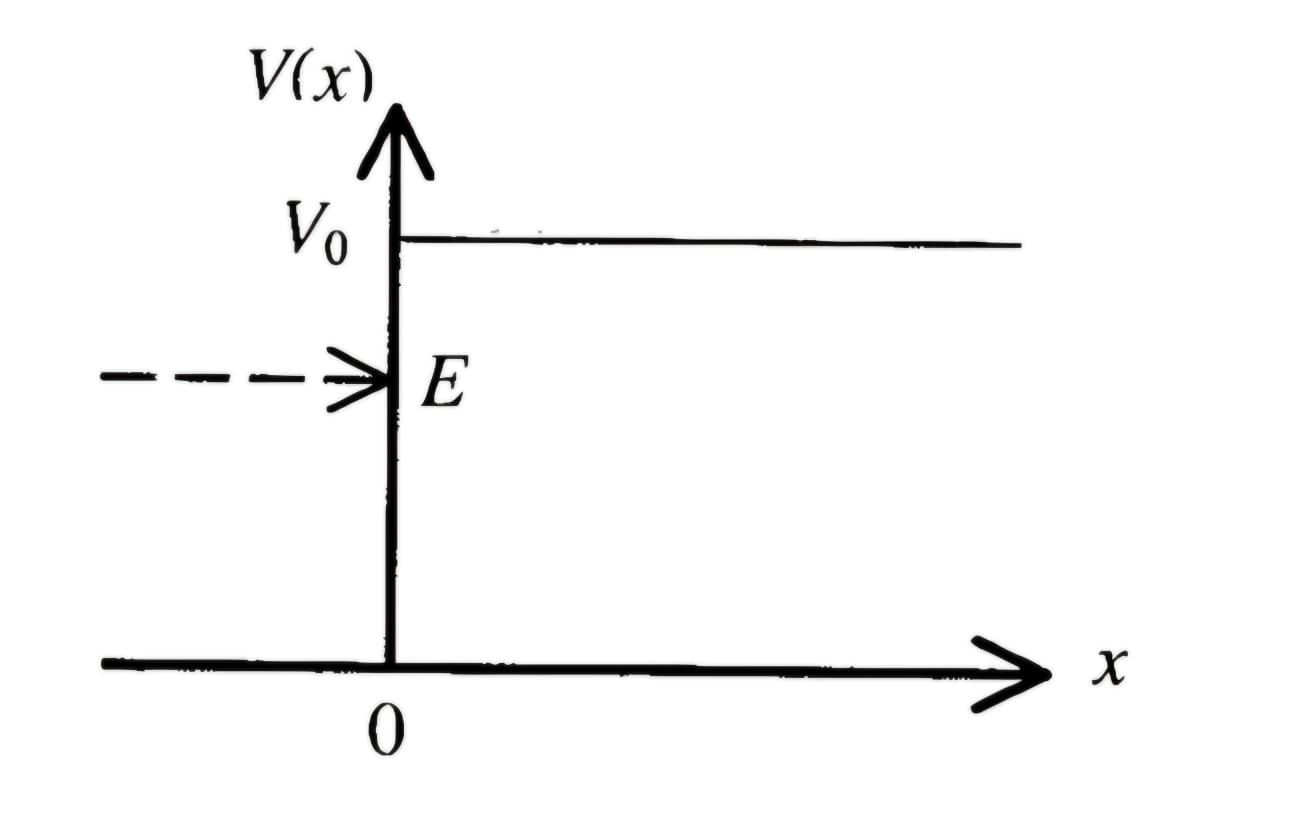
\includegraphics[width=0.35\textwidth]{fig1.jpeg}
    \caption{}
    \label{fig:fig1.jpeg}
\end{figure}

For $E<V_0$, the space part of the wavefunction for $x>0$ is of the form

\hfill{\brak{\text{GATE IN 2011}}}

\begin{multicols}{4}
\begin{enumerate}
    \item $e^{\alpha x}$
    \item $e^{-\alpha x}$
    \item $e^{i\alpha x}$
    \item $e^{-i\alpha x}$
\end{enumerate}
\end{multicols}

\item If $L_{x}$, $L_{y}$ and $L_{z}$ are respectively the $x$, $y$ and $z$ components of the angular momentum operator $\vec{L}$, the commutator $[L_{z} L_{x}, L_{z}]$ is equal to

\hfill{\brak{\text{GATE IN 2011}}}

\begin{multicols}{4}
\begin{enumerate}
    \item $i\hbar \left(L_{x}^{3} + L_{y}^{2}\right)$
    \item $2 i \hbar L_{z}$
    \item $i\hbar \left(L_{x}^{2} - L_{y}^{2}\right)$
    \item $0$
\end{enumerate}
\end{multicols}

\item The normalized ground state wavefunction of a hydrogen atom is given by $\psi(r) = \frac{1}{\sqrt{4\pi}} \cdot \frac{2}{a^{5/2}} \ e^{-r/a}$
where $a$ is the Bohr radius and $r$ is the distance of the electron from the nucleus, located at the origin.  
The expectation value $\langle \dfrac{1}{r^{2}} \rangle$ is

\hfill{\brak{\text{GATE IN 2011}}}

\begin{multicols}{4}
\begin{enumerate}
    \item $\dfrac{8\pi}{a^{2}}$
    \item $\dfrac{4\pi}{a^{2}}$
    \item $\dfrac{4}{a^{2}}$
    \item $\dfrac{2}{a^{2}}$
\end{enumerate}
\end{multicols}

\item Two charges $q$ and $2q$ are placed along the $x$-axis in front of a grounded, infinite conducting plane, as shown in the figure. They are located respectively at a distance of $0.5 \ \mathrm{m}$ and $1.5 \ \mathrm{m}$ from the plane. The force acting on the charge $q$ is



\begin{figure}[ht!]
    \centering
    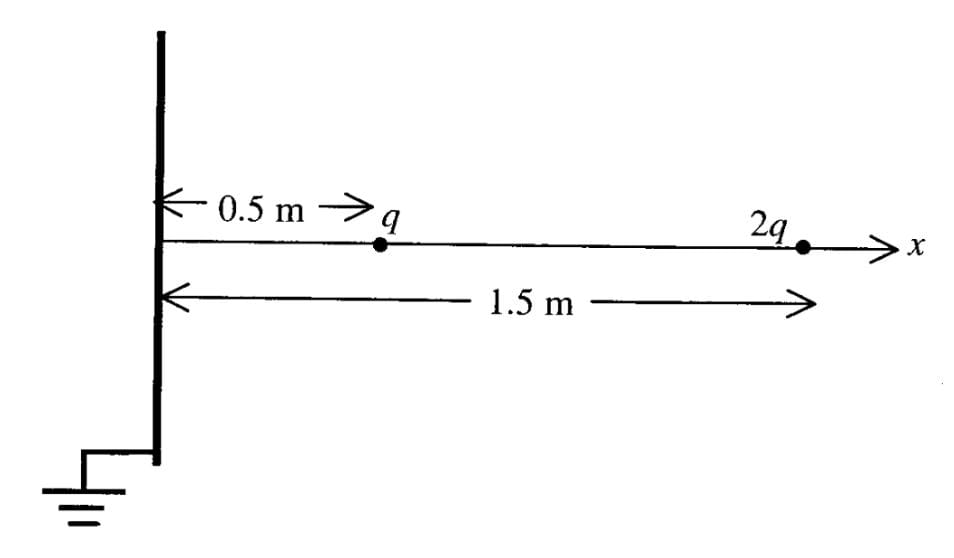
\includegraphics[width=0.5\textwidth]{fig2.jpeg}
    \caption{}
    \label{fig:fig2.jpeg}
\end{figure}

\hfill{\brak{\text{GATE IN 2011}}}

\begin{multicols}{4}
\begin{enumerate}
    \item $\dfrac{1}{4\pi\epsilon_{0}} \cdot \dfrac{7q^{2}}{2}$
    \item $\dfrac{1}{4\pi\epsilon_{0}} \cdot 2q^{2}$
    \item $\dfrac{1}{4\pi\epsilon_{0}} \cdot q^{2}$
    \item $\dfrac{1}{4\pi\epsilon_{0}} \cdot \dfrac{q^{2}}{2}$
\end{enumerate}
\end{multicols}

\item A uniform surface current is flowing in the positive $y$-direction over an infinite sheet lying in $x$-$y$ plane. The direction of the magnetic field is  

\hfill{\brak{\text{GATE IN 2011}}}

\begin{multicols}{2}
\begin{enumerate}
    \item along $\hat{i}$ for $z > 0$ and along $-$ for $z < 0$
    \item along for $z > 0$ and along $\hat{k}$ for $z < 0$
    \item along $-\hat{i}$ for $z > 0$ and along \dots
    \item along $-\hat{k}$
\end{enumerate}
\end{multicols}

\item A magnetic dipole of dipole moment $\vec{m}$ is placed in a non-uniform magnetic field $\vec{B}$. If the position vector of the dipole is $\overline{r}$, the torque acting on the dipole about the origin is  

\hfill{\brak{\text{GATE IN 2011}}}

\begin{multicols}{2}
\begin{enumerate}
    \item $\vec{r} \times (\vec{m} \times \vec{B})$
    \item $\vec{r} \times \vec{\nabla} (\vec{m} \cdot \vec{B})$
    \item $\vec{m} \times \vec{B}$
    \item $\vec{m} \times \vec{B} + \vec{r} \times \vec{\nabla} (\vec{m} \cdot \vec{B})$
\end{enumerate}
\end{multicols}

\item Which of the following expressions for a vector potential $\vec{A}$ \textbf{does not} represent a uniform magnetic field of magnitude $B_{0}$ along the $z$-direction?  

\hfill{\brak{\text{GATE IN 2011}}}

\begin{multicols}{2}
\begin{enumerate}
    \item $\overline{A} = (0, B_{0}x, 0)$
    \item $\overline{A} = (-B_{0}y, 0, 0)$
    \item $\vec{A} = \left( \frac{B_{0}x}{2}, \frac{B_{0}y}{2}, 0 \right)$
    \item $\vec{A} = \left( -\frac{B_{0}y}{2}, \frac{B_{0}x}{2}, 0 \right)$
\end{enumerate}
\end{multicols}

\item A neutron passing through a detector is detected because of  

\hfill{\brak{\text{GATE IN 2011}}}


\begin{enumerate}
    \item the ionization it produces
    \item the scintillation light it produces
    \item the electron-hole pairs it produces
    \item the secondary particles produced in a nuclear reaction in the detector medium
\end{enumerate}


\item An atom with one outer electron having orbital angular momentum $l$ is placed in a weak magnetic field. The number of energy levels into which the higher total angular momentum state splits, is  

\hfill{\brak{\text{GATE IN 2011}}}

\begin{multicols}{2}
\begin{enumerate}
    \item $2l+2$
    \item $2l+1$
    \item $2l$
    \item $2l-1$
\end{enumerate}
\end{multicols}

\item For a multi-electron atom, $l$, $L$, and $S$ specify the one-electron orbital angular momentum, total orbital angular momentum, and total spin angular momentum, respectively. The selection rules for electric dipole transition between the two electronic energy levels, specified by $l$, $L$, and $S$ are  

\hfill{\brak{\text{GATE IN 2011}}}

\begin{multicols}{2}
\begin{enumerate}
    \item $\Delta L = 0, \pm 1;\ \Delta l = 0, \pm 1;\ \Delta S = 0$
    \item $\Delta l = 0, \pm 1;\ \Delta S = 0;\ \Delta L = \pm 1$
    \item $\Delta L = 0, 1;\ \Delta S = \pm 1;\ \Delta l = 0, \pm 1$
    \item $\Delta L = 0;\ \Delta S = \pm 1;\ \Delta l = \pm 1$
\end{enumerate}
\end{multicols}

\item For a three-dimensional crystal having $N$ primitive unit cells with a basis of $p$ atoms, the number of optical branches is  

\hfill{\brak{\text{GATE IN 2011}}}

\begin{multicols}{4}
\begin{enumerate}
    \item $3$
    \item $3p$
    \item $3p - 3$
    \item $3N - 3p$
\end{enumerate}
\end{multicols}

\item For an intrinsic semiconductor, $m_{e}^{}$ and $m_{h}^{}$ are respectively the effective masses of electrons and holes near the corresponding band edges. At a finite temperature, the position of the Fermi level  

\hfill{\brak{\text{GATE IN 2011}}}

\begin{enumerate}
    \item depends on $m_{e}^{}$ but not on $m_{h}^{}$
    \item depends on $m_{h}^{}$ but not on $m_{e}^{}$
    \item depends on both $m_{e}^{}$ and $m_{h}^{}$
    \item depends neither on $m_{e}^{}$ nor on $m_{h}^{}$
\end{enumerate}

\item In the following circuit, the voltage across and the current through 2k\ohm resistance are

\begin{figure}[ht!]
    \centering
    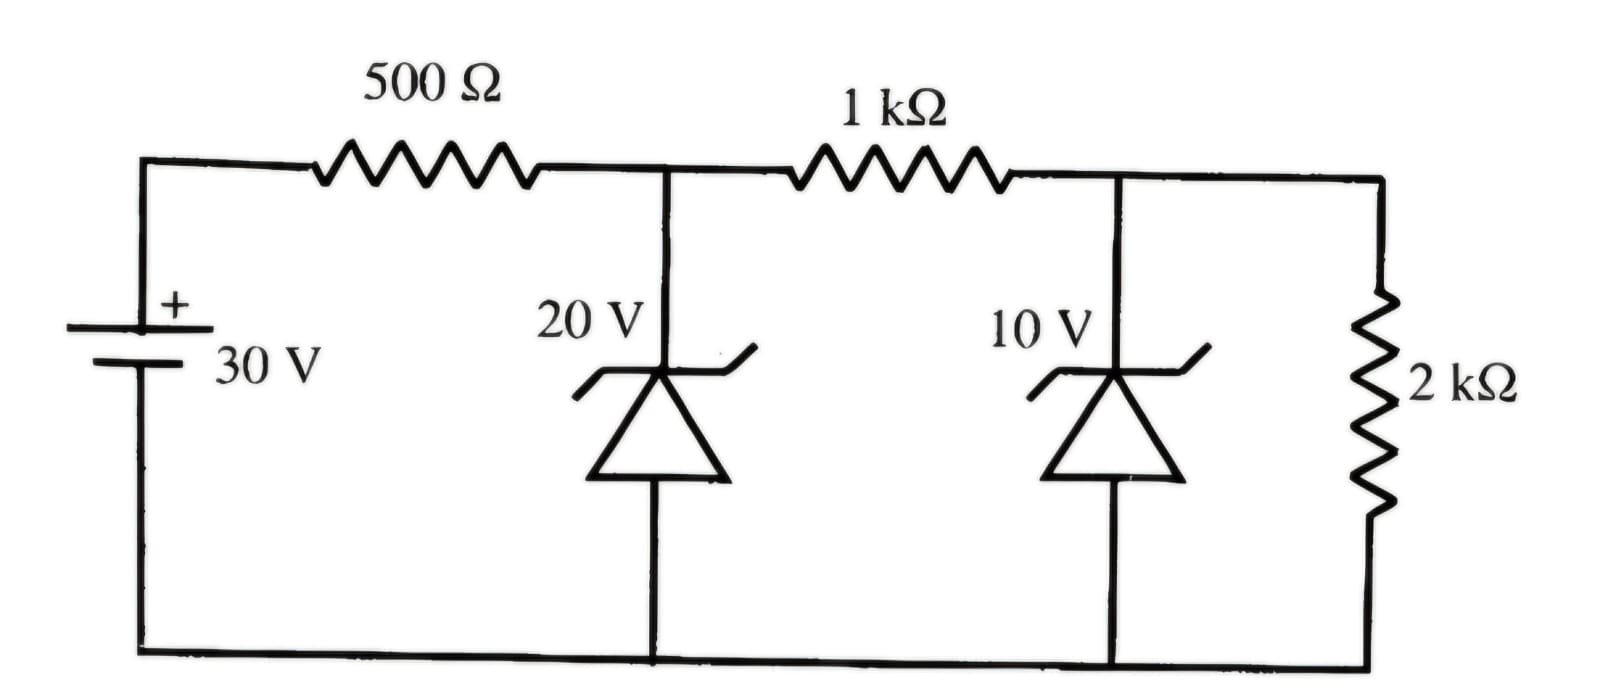
\includegraphics[width=0.5\textwidth]{fig3.jpeg}
    \caption{}
    \label{fig:fig3.jpeg}
\end{figure}

\hfill{\brak{\text{GATE IN 2011}}}

\begin{multicols}{4}
\begin{enumerate}
    \item 20V, 10mA
    \item 20V, 5mA
    \item 10V, 10mA
    \item 10V, 5mA
\end{enumerate}
\end{multicols}


\item The unit vector normal to the surface $x^{2} + y^{2} - z = 1$ at the point $P(1,1,1)$ is 

\hfill{\brak{\text{GATE IN 2011}}}

\begin{multicols}{4}
\begin{enumerate}
    \item $\dfrac{\hat{i} + \hat{j} - \hat{k}}{\sqrt{3}}$
    \item $\dfrac{2\hat{i} + \hat{j} - \hat{k}}{\sqrt{6}}$
    \item $\dfrac{\hat{i} + 2\hat{j} - \hat{k}}{\sqrt{6}}$
    \item $\dfrac{2\hat{i} + 2\hat{j} - \hat{k}}{3}$
\end{enumerate}
\end{multicols}

\item Consider a cylinder of height $h$ and radius $a$, closed at both ends, centered at the origin.  
Let $\vec{r} = \hat{i}x + \hat{j}y + \hat{k}z$ be the position vector and $\hat{n}$ a unit vector normal to the surface.  
The surface integral $\int_{S} \vec{r} \cdot \hat{n} \, dS$ over the closed surface of the cylinder is

\begin{figure}[ht!]
    \centering
    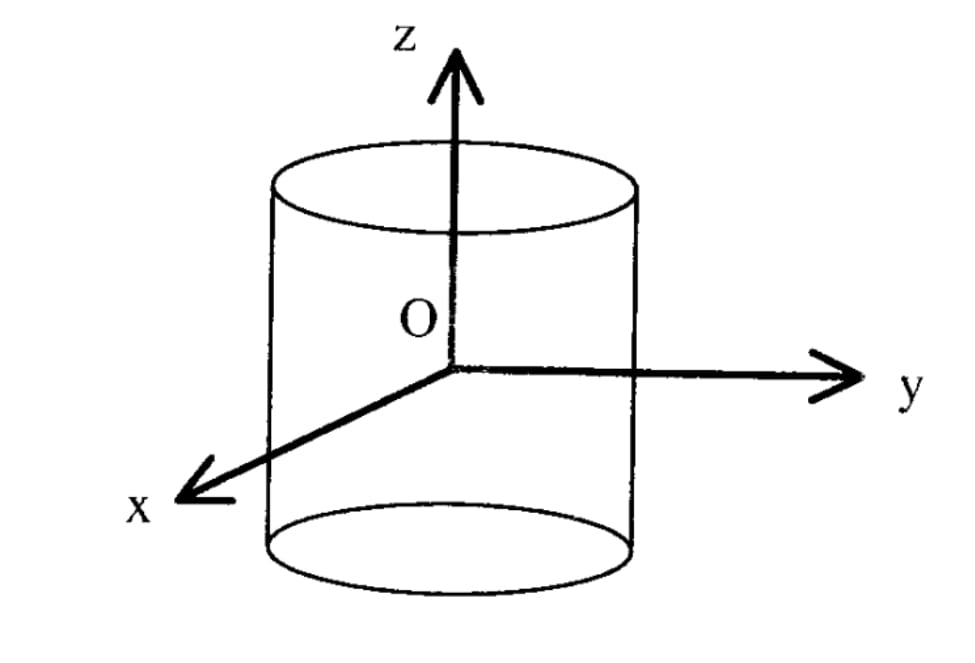
\includegraphics[width=0.3\textwidth]{fig4.jpeg}
    \caption{}
    \label{fig:fig4.jpeg}
\end{figure}

\hfill{\brak{\text{GATE IN 2011}}}


\begin{multicols}{4}
\begin{enumerate}
    \item $2\pi a^2 \brak{a + h}$
    \item $3\pi a^2 h$
    \item $2\pi a^2 h$
    \item zero
\end{enumerate}
\end{multicols}


\item The solutions to the differential equation $\frac{dy}{dx} = -\frac{x}{y + 1}$
are a family of  

\hfill{\brak{\text{GATE IN 2011}}}

\begin{enumerate}
    \item circles with different radii
    \item circles with different centres
    \item straight lines with different slopes
    \item straight lines with different intercepts on the y-axis
\end{enumerate}

\item A particle is moving under the action of a generalized potential. The magnitude of the generalized force is  

\hfill{\brak{\text{GATE IN 2011}}}

\begin{multicols}{4}
\begin{enumerate}
    \item $2(1+q)$
    \item $2(1-q)$
    \item $2q$
    \item $4q$
\end{enumerate}
\end{multicols}

\item Two bodies of mass $m$ and $2m$ are connected by a spring of spring constant $k$. The frequency of the normal mode is   

\hfill{\brak{\text{GATE IN 2011}}}

\begin{multicols}{4}
\begin{enumerate}
    \item $\sqrt{\frac{3k}{2m}}$
    \item $\sqrt{\frac{k}{m}}$
    \item $\sqrt{\frac{2k}{3m}}$
    \item $\sqrt{\frac{k}{2m}}$
\end{enumerate}
\end{multicols}

\item Let $(q,p)$ and $(Q,P)$ be two pairs of canonical variables. The transformation $Q = q^{\alpha} \cos(\beta p)$ is canonical for $P = q^{\alpha} \sin(\beta p)$.  

\hfill{\brak{\text{GATE IN 2011}}}

\begin{multicols}{4}
\begin{enumerate}
    \item $\beta = \frac12, \ \alpha = 2$
    \item $\alpha = 2, \ \beta = 2$
    \item $\alpha = 1, \ \beta = 1$
    \item $\beta = 2, \ \alpha = \frac12$
\end{enumerate}
\end{multicols}

\item Two particles, each of rest mass $m$, collide head-on and stick together. Before collision, the speed of each mass was $0.6$ times the speed of light in free space. The mass of the final entity is 

\hfill{\brak{\text{GATE IN 2011}}}

\begin{multicols}{4}
\begin{enumerate}
    \item $\frac{5m}{4}$
    \item $2m$
    \item $\frac{5m}{2}$
    \item $\frac{25m}{8}$
\end{enumerate}
\end{multicols}

\item The normalized eigenstates of a particle in a one-dimensional potential well are given by  
\[
V(x) = 
\begin{cases}
0, & 0 \le x \le a \\
\infty, & \text{otherwise}
\end{cases}
\]
where $n = 1,2,3,\dots$ and  
\[
\psi_{n}(x) = \sqrt{\frac{2}{a}} \sin\left( \frac{n\pi x}{a} \right)
\]
The particle is subjected to  
\[
V'(x) = 
\begin{cases}
V_{0} \cos\left( \frac{\pi x}{a} \right), & 0 \le x \le \frac{a}{2} \\
0, & \text{otherwise}
\end{cases}
\]
The shift in the ground state energy due to the perturbation, in the first order perturbation theory, is  

\hfill{\brak{\text{GATE IN 2011}}}

\begin{multicols}{4}
\begin{enumerate}
    \item $\frac{2V_{0}}{3\pi}$
    \item $\frac{V_{0}}{3\pi}$
    \item $-\frac{V_{0}}{3\pi}$
    \item $-\frac{2V_{0}}{3\pi}$
\end{enumerate}
\end{multicols}

\item If the isothermal compressibility of a solid is $10^{-10} \ \mathrm{Pa}^{-1}$, the pressure required to increase its density by $1\%$ is approximately:

\hfill{\brak{\text{GATE IN 2011}}}

\begin{multicols}{4}
\begin{enumerate}
    \item $10^{4} \ \mathrm{Pa}$
    \item $10^{6} \ \mathrm{Pa}$
    \item $10^{8} \ \mathrm{Pa}$
    \item $10^{10} \ \mathrm{Pa}$
\end{enumerate}
\end{multicols}

\item A system of $N$ non-interacting and distinguishable particles of spin $1$ is in thermodynamic equilibrium. The entropy of the system is:

\hfill{\brak{\text{GATE IN 2011}}}

\begin{multicols}{4}
\begin{enumerate}
    \item $2 k_{B} \ln N$
    \item $3 k_{B} N$
    \item $2 N k_{B}$
    \item $N k_{B} \ln 3$
\end{enumerate}
\end{multicols}

\item A system has two energy levels with energies $x$ and $2x$. The lower level is 4-fold degenerate while the upper level is doubly degenerate. If there are $N$ non-interacting classical particles in the system, which is in thermodynamic equilibrium at a temperature $T$, the fraction of particles in the upper level is:

\hfill{\brak{\text{GATE IN 2011}}}

\begin{multicols}{2}
\begin{enumerate}
    \item $\dfrac{1}{1 + e^{(-x)/(k_{B}T)}}$
    \item $\dfrac{1}{1 + 2 e^{x/(k_{B}T)}}$
    \item $\dfrac{1}{2 e^{x/(k_{B}T)} + 4 e^{2x/(k_{B}T)}}$
    \item $\dfrac{1}{2 e^{x/(k_{B}T)} - 4 e^{2x/(k_{B}T)}}$
\end{enumerate}
\end{multicols}

\item A spherical conductor of radius $a$ is placed in a uniform electric field $\overline{E} = E_{0} \hat{k}$. The potential at a point $P(r,\theta)$ for $r > a$ is given by:
\[
\varphi(r,\theta) = \text{constant} - E_{0} r \cos\theta + \frac{E_{0} a^{3}}{r^{2}} \cos\theta
\]
where $r$ is the distance from the origin and $\theta$ is the angle $OP$ makes with the $z$-axis.


\begin{figure}[ht!]
    \centering
    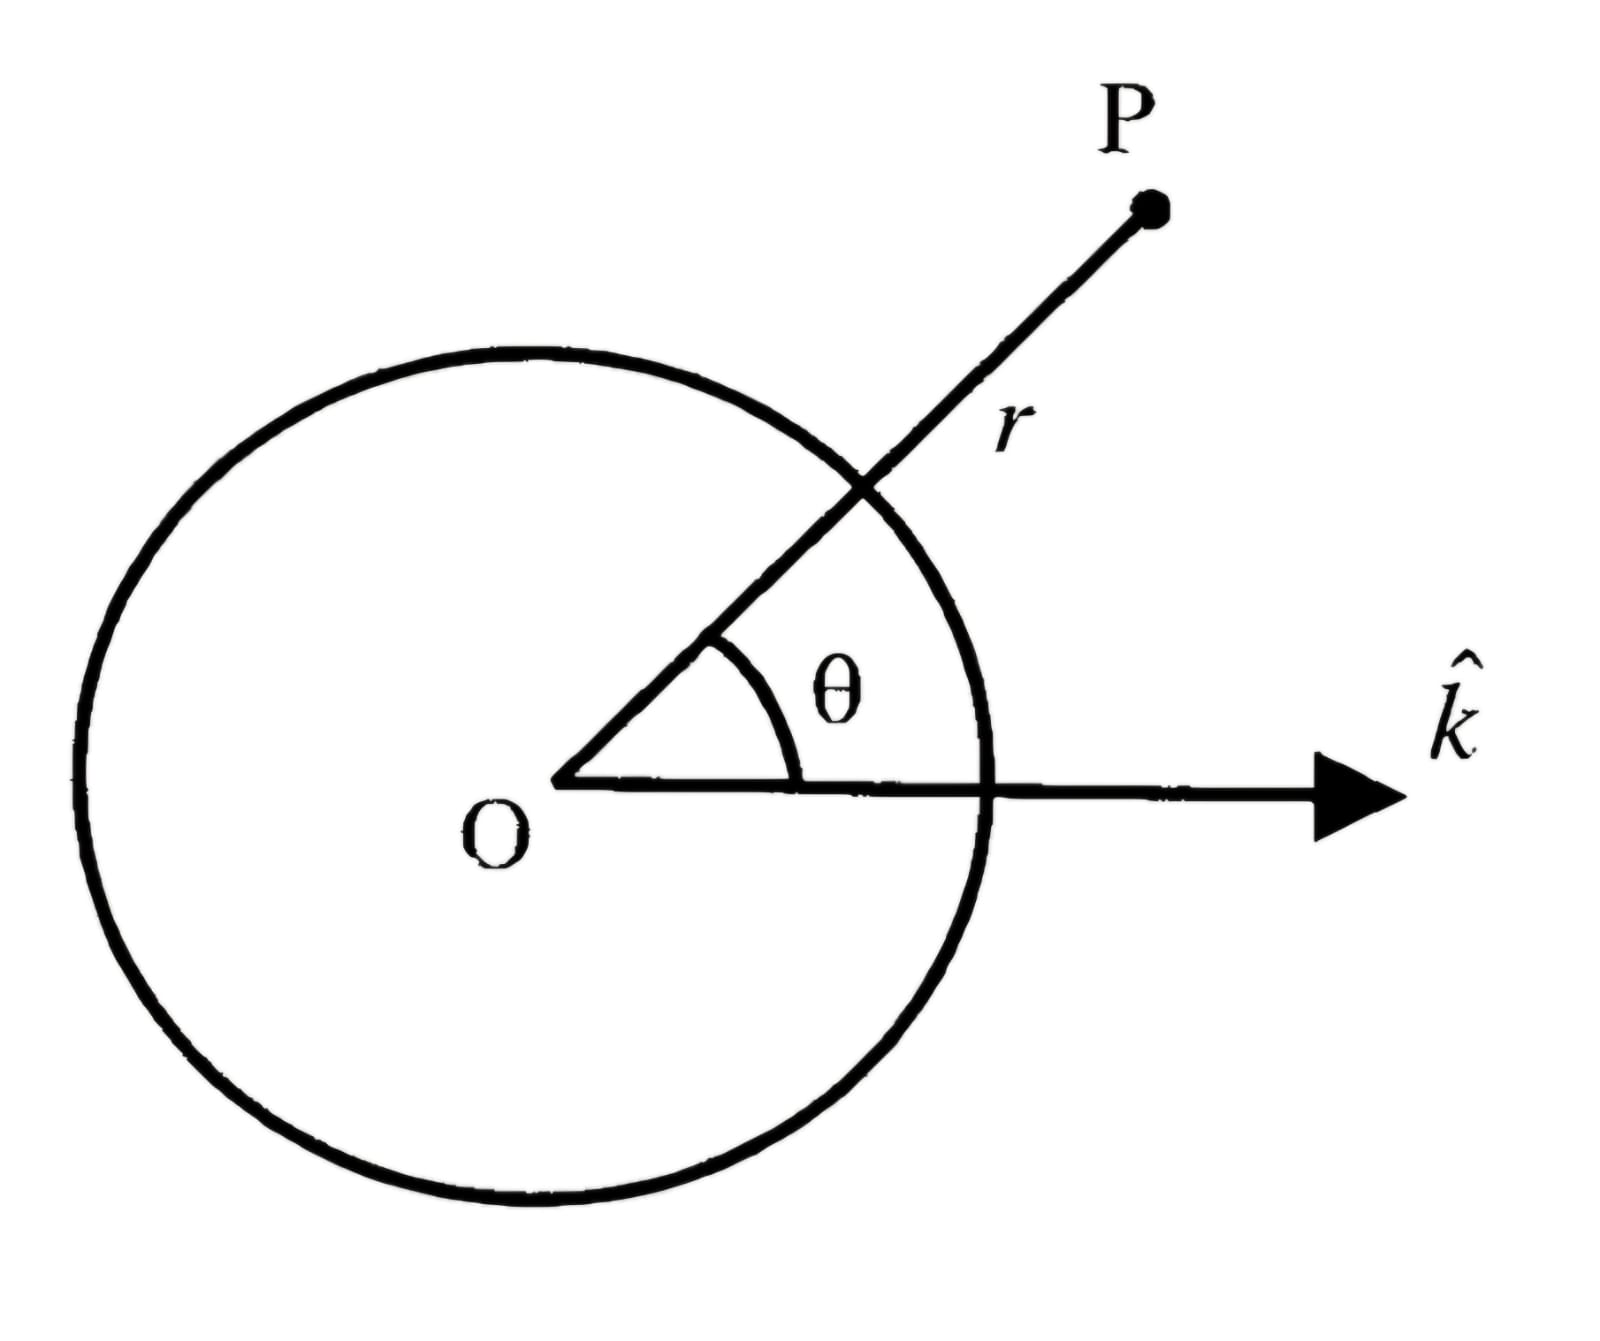
\includegraphics[width=0.35\textwidth]{fig5.jpeg}
    \caption{}
    \label{fig:fig5.jpeg}
\end{figure}


The charge density on the sphere at $\theta = 30^\circ$ is:

\hfill{\brak{\text{GATE IN 2011}}}

\begin{multicols}{4}
\begin{enumerate}
    \item $\dfrac{3\sqrt{3} \ \epsilon_{0} E_{0}}{2}$
    \item $\dfrac{3 \ \epsilon_{0} E_{0}}{2}$
    \item $\dfrac{\sqrt{3} \ \epsilon_{0} E_{0}}{2}$
    \item $\dfrac{\epsilon_{0} E_{0}}{2}$
\end{enumerate}
\end{multicols}

\item According to the single particle nuclear shell model, the spin-parity of the ground state of ${}^{17}_{8}\mathrm{O}$ is:

\hfill{\brak{\text{GATE IN 2011}}}

\begin{multicols}{4}
\begin{enumerate}
    \item $\dfrac{1}{2}^-$
    \item $\dfrac{3}{2}^-$
    \item $\dfrac{3}{2}^+$
    \item $\dfrac{5}{2}^+$
\end{enumerate}
\end{multicols}

\item In the $\beta$-decay of neutron $n \rightarrow p + e^- + \bar{\nu}_e$, the anti-neutrino escapes detection. Its existence is inferred from the measurement of:

\hfill{\brak{\text{GATE IN 2011}}}

\begin{multicols}{2}
\begin{enumerate}
    \item Energy distribution of electrons
    \item Angular distribution of electrons
    \item Helicity distribution of electrons
    \item Forward-backward asymmetry of electrons
\end{enumerate}
\end{multicols}

\item The isospin and the strangeness of $\Omega^-$ baryon are:

\hfill{\brak{\text{GATE IN 2011}}}

\begin{multicols}{4}
\begin{enumerate}
    \item $1, -3$
    \item $0, -3$
    \item $1, 3$
    \item $0, 3$
\end{enumerate}
\end{multicols}

\item The lifetime of an atomic state is $1\,\mathrm{ns}$. The natural line width of the spectral line in the emission spectrum of this state is of the order of:

\hfill{\brak{\text{GATE IN 2011}}}

\begin{multicols}{4}
\begin{enumerate}
    \item $10^{-1} \,\mathrm{eV}$
    \item $10^{-3} \,\mathrm{eV}$
    \item $10^{-5} \,\mathrm{eV}$
    \item $10^{-7} \,\mathrm{eV}$
\end{enumerate}
\end{multicols}

\item The degeneracy of an excited state of nitrogen atom having electronic configuration $1s^2 \, 2s^2 \, 2p^3 \, 3d^1$:

\hfill{\brak{\text{GATE IN 2011}}}

\begin{multicols}{4}
\begin{enumerate}
    \item 6
    \item 10
    \item 15
    \item 150
\end{enumerate}
\end{multicols}

\item The far infrared rotational absorption spectrum of a diatomic molecule shows equidistant lines with spacing $20\,\mathrm{cm^{-1}}$. The position of the first Stokes line in the rotational Raman spectrum of this molecule is:

\hfill{\brak{\text{GATE IN 2011}}}

\begin{multicols}{4}
\begin{enumerate}
    \item $20\,\mathrm{cm^{-1}}$
    \item $40\,\mathrm{cm^{-1}}$
    \item $60\,\mathrm{cm^{-1}}$
    \item $120\,\mathrm{cm^{-1}}$
\end{enumerate}
\end{multicols}

\item A metal with body-centered cubic (bcc) structure shows the first (smallest angle) diffraction peak at a Bragg angle $\theta = 30^\circ$. The wavelength of X-ray used is $2.1\,\text{\AA}$. The volume of the primitive unit cell of the metal is:

\hfill{\brak{\text{GATE IN 2011}}}

\begin{multicols}{4}
\begin{enumerate}
    \item $26.2\,\text{\AA}^3$
    \item $13.1\,\text{\AA}^3$
    \item $9.3\,\text{\AA}^3$
    \item $4.6\,\text{\AA}^3$
\end{enumerate}
\end{multicols}

\item In the following circuit, Tr$1$ and Tr$_2$ are identical transistors having $V{BE} = 0.7\,\mathrm{V}$. The current passing through transistor Tr$_2$ is:

\begin{figure}[ht!]
    \centering
    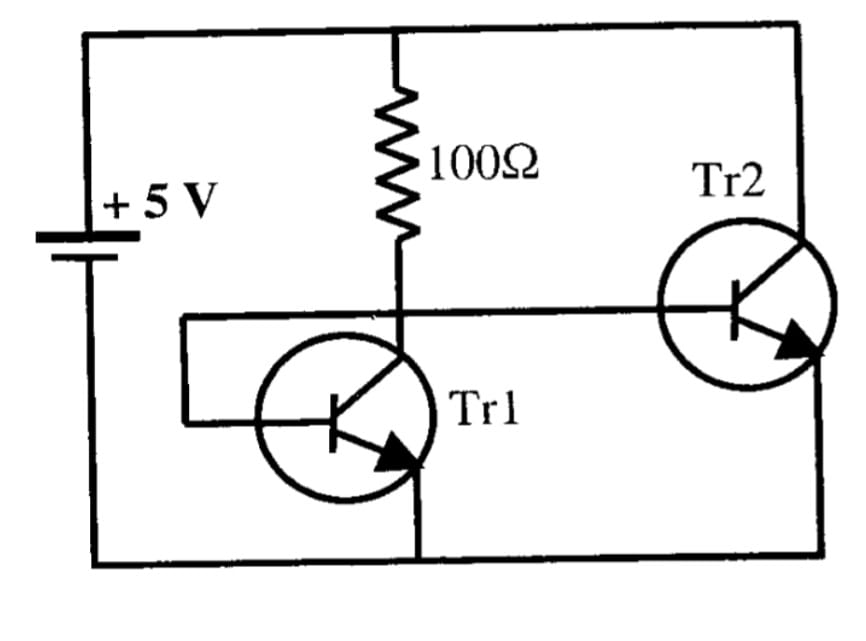
\includegraphics[width=0.3\textwidth]{fig6.jpeg}
    \caption{}
    \label{fig:fig6.jpeg}
\end{figure}


\hfill{\brak{\text{GATE IN 2011}}}

\begin{multicols}{4}
\begin{enumerate}
    \item $57\,\mathrm{mA}$
    \item $50\,\mathrm{mA}$
    \item $48\,\mathrm{mA}$
    \item $43\,\mathrm{mA}$
\end{enumerate}
\end{multicols}

\item The following Boolean expression 
\[
Y = A\overline{B} \, \overline{C} \, \overline{D} 
+ \overline{A}B \, \overline{C} D
+ \overline{A} \, \overline{B} \, \overline{C} D
+ \overline{A} \, \overline{B} C D
+ \overline{A} B C D
+ A \, \overline{B} \, \overline{C} D
\]
can be simplified into:


\hfill{\brak{\text{GATE IN 2011}}}


\begin{multicols}{2}
\begin{enumerate}
    \item $\overline{A} \, \overline{B} C + A \, \overline{D}$
    \item $\overline{A} B \, \overline{C} + A \, \overline{D}$
    \item $A \, \overline{B} \, \overline{C} + \overline{A} D$
    \item $A \, \overline{B} C + \overline{A} D$
\end{enumerate}
\end{multicols}

\item Consider the following circuit.

\begin{figure}[ht!]
    \centering
    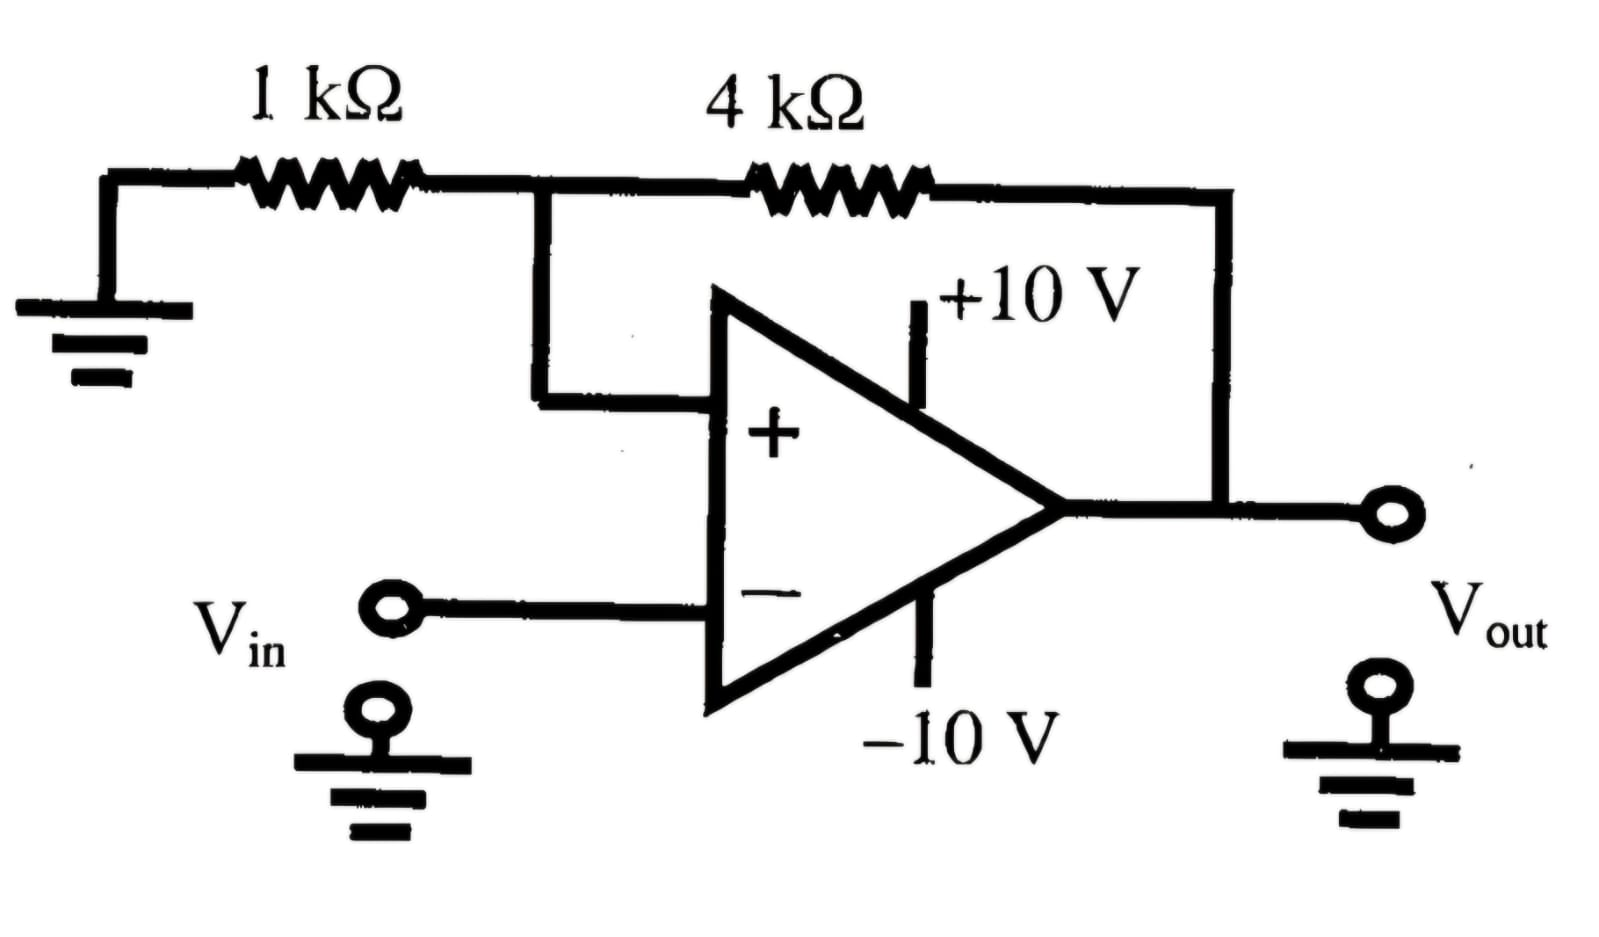
\includegraphics[width=0.6\textwidth]{fig7.jpeg}
    \caption{}
    \label{fig:fig7.jpeg}
\end{figure}

Which of the following correctly represents the output V\text{out} corresponding to the input V\text{in} ?

\hfill{\brak{\text{GATE IN 2011}}}

\begin{multicols}{2}
\begin{enumerate}
    \item 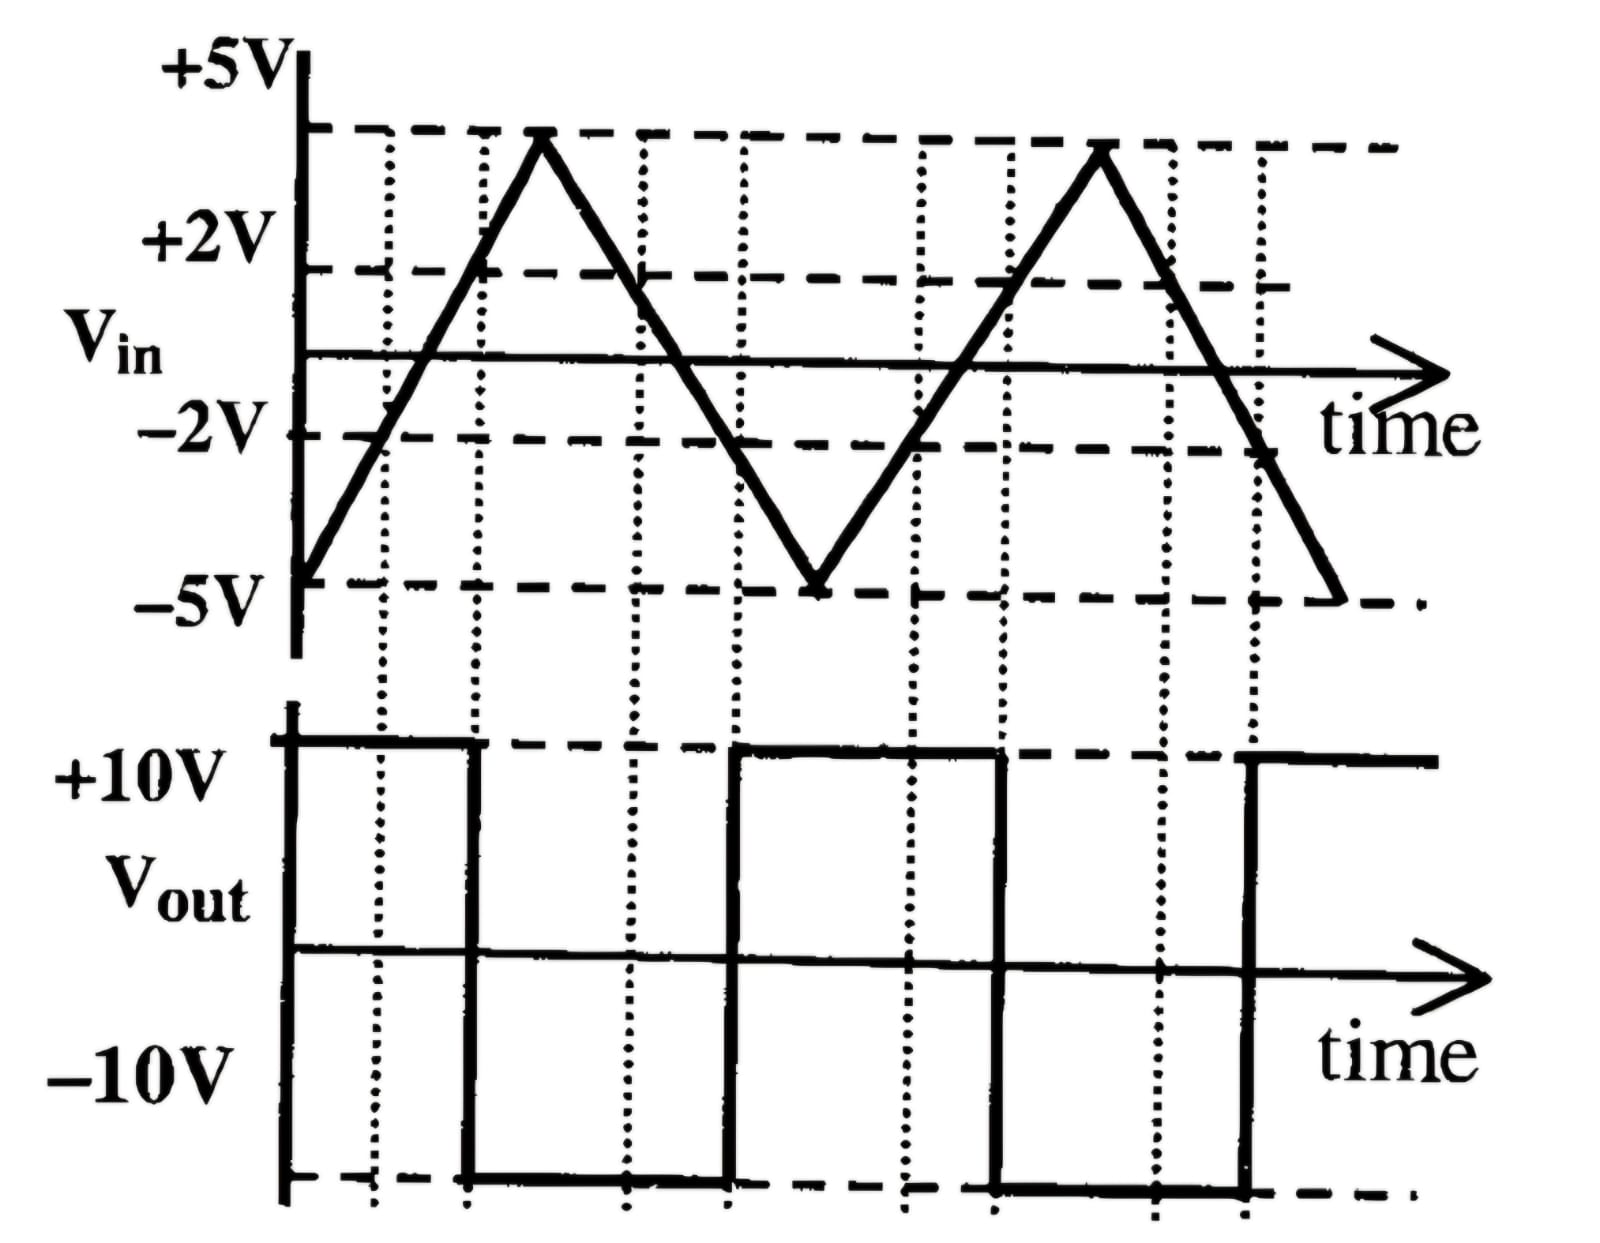
\includegraphics[width=0.25\textwidth]{fig8.jpeg} \hfill
    \item 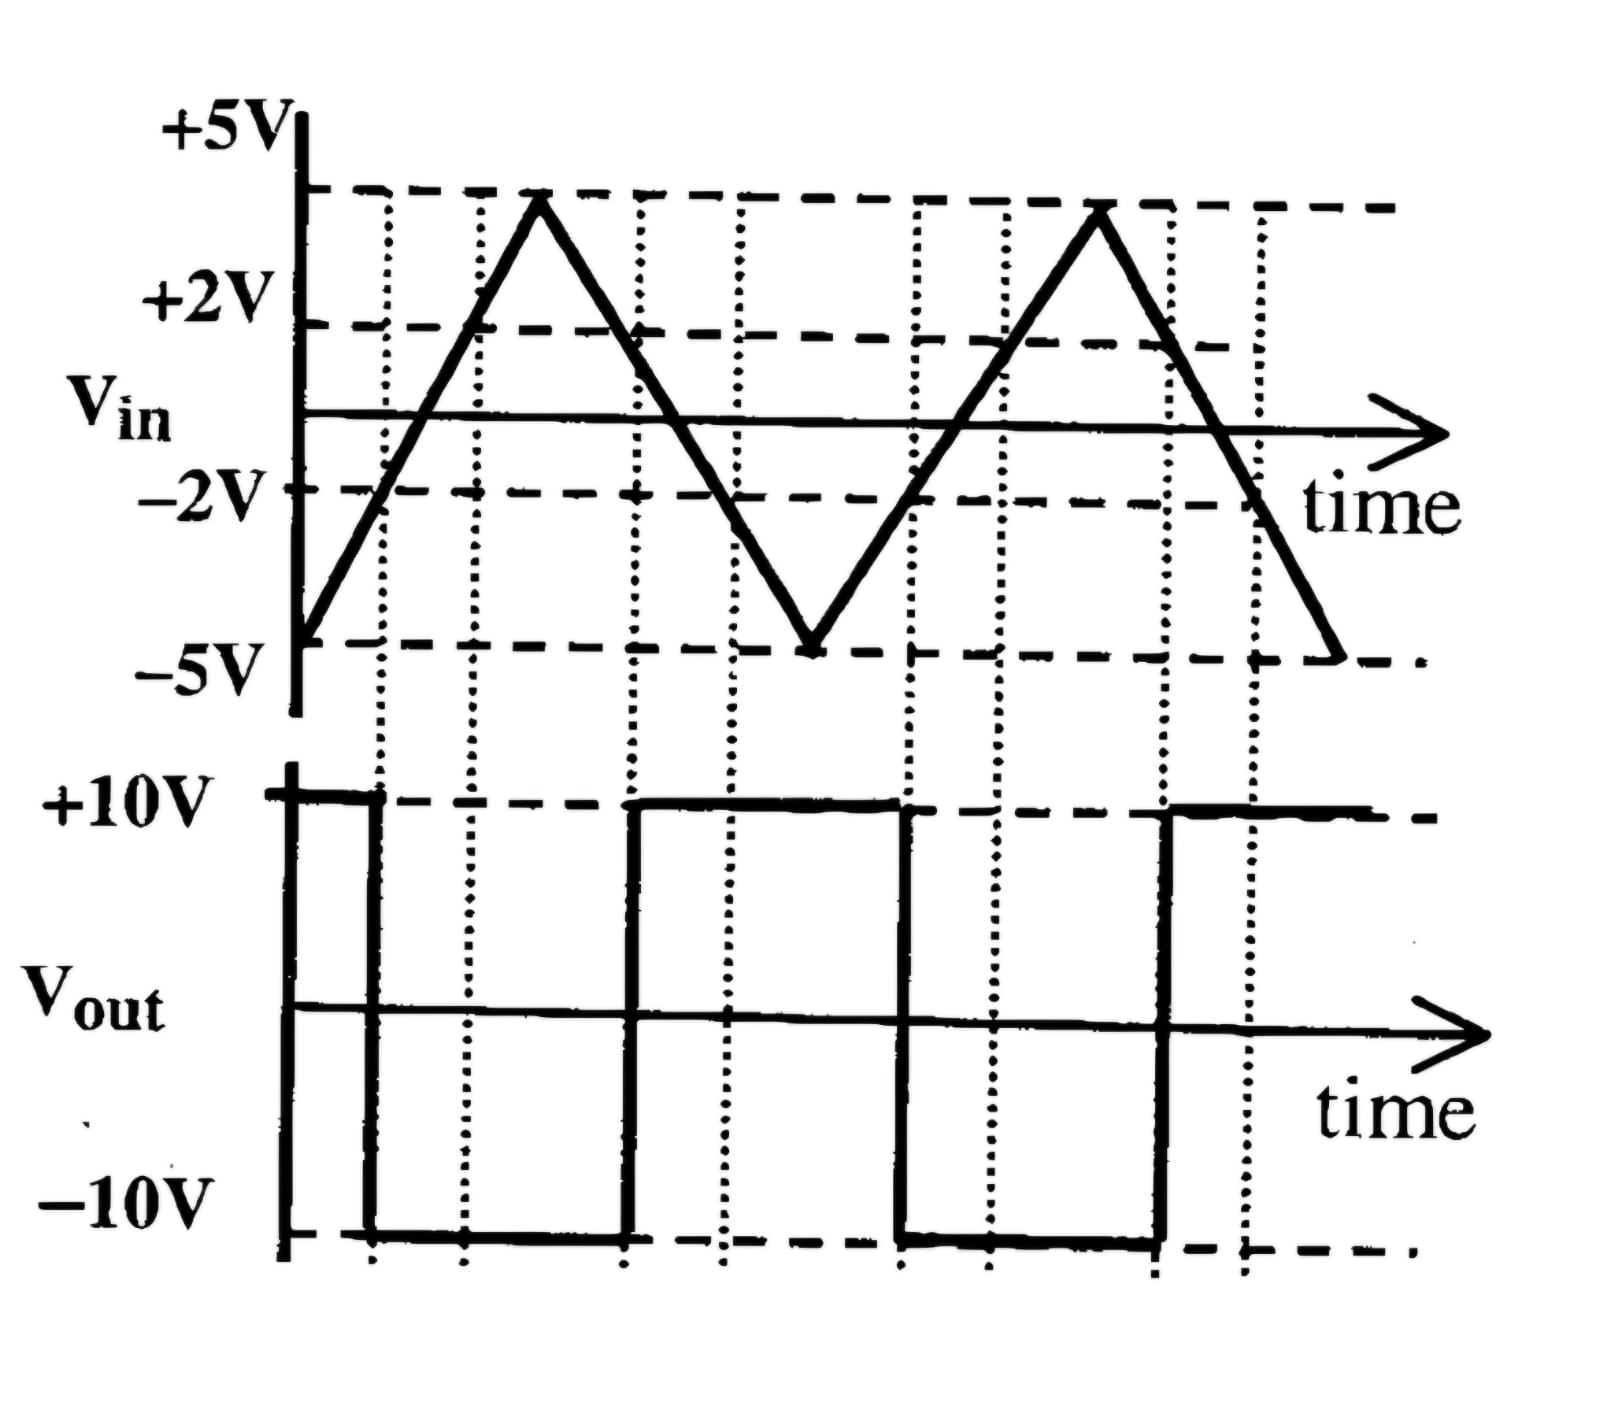
\includegraphics[width=0.25\textwidth]{fig9.jpeg} \hfill
    \item 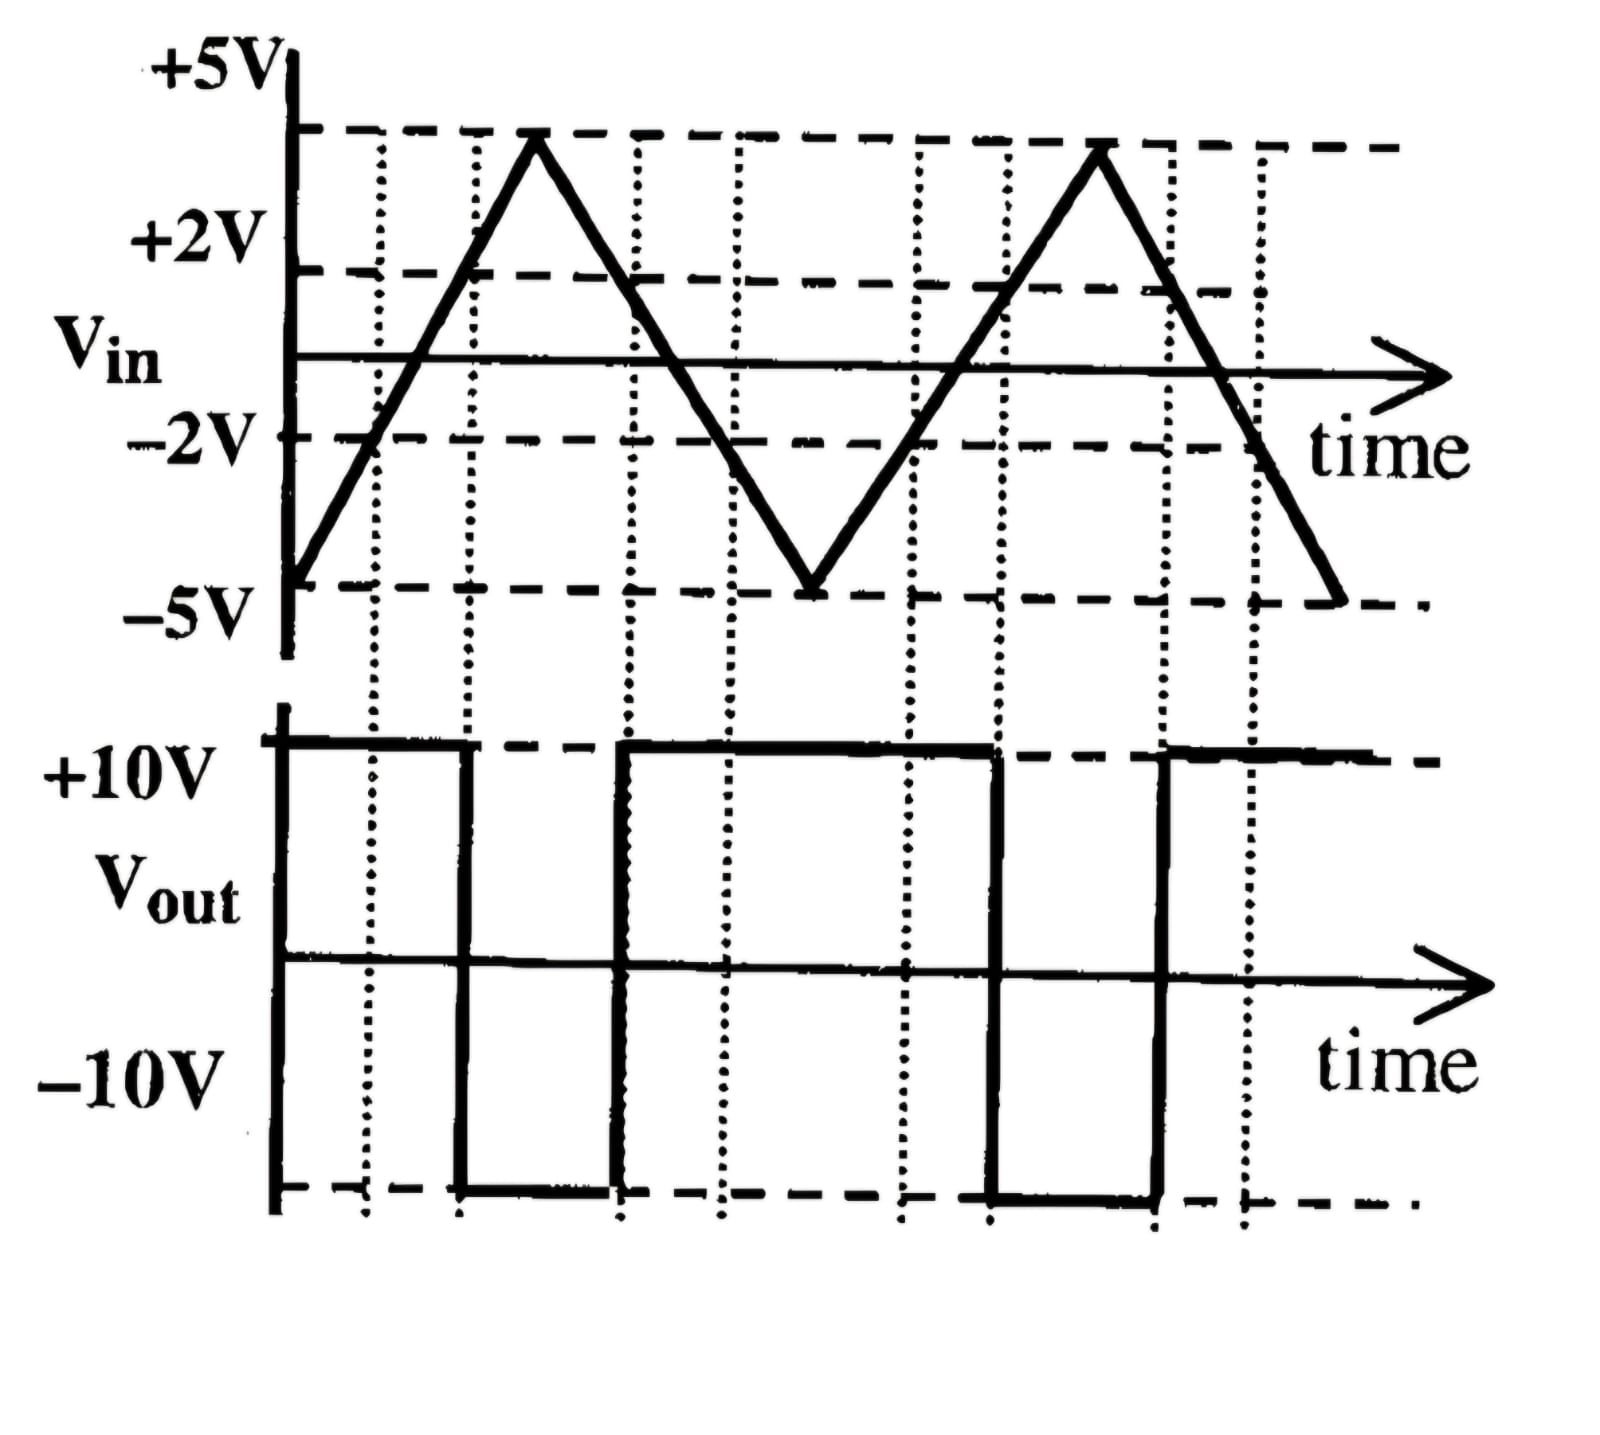
\includegraphics[width=0.25\textwidth]{fig10.jpeg} \hfill
    \item 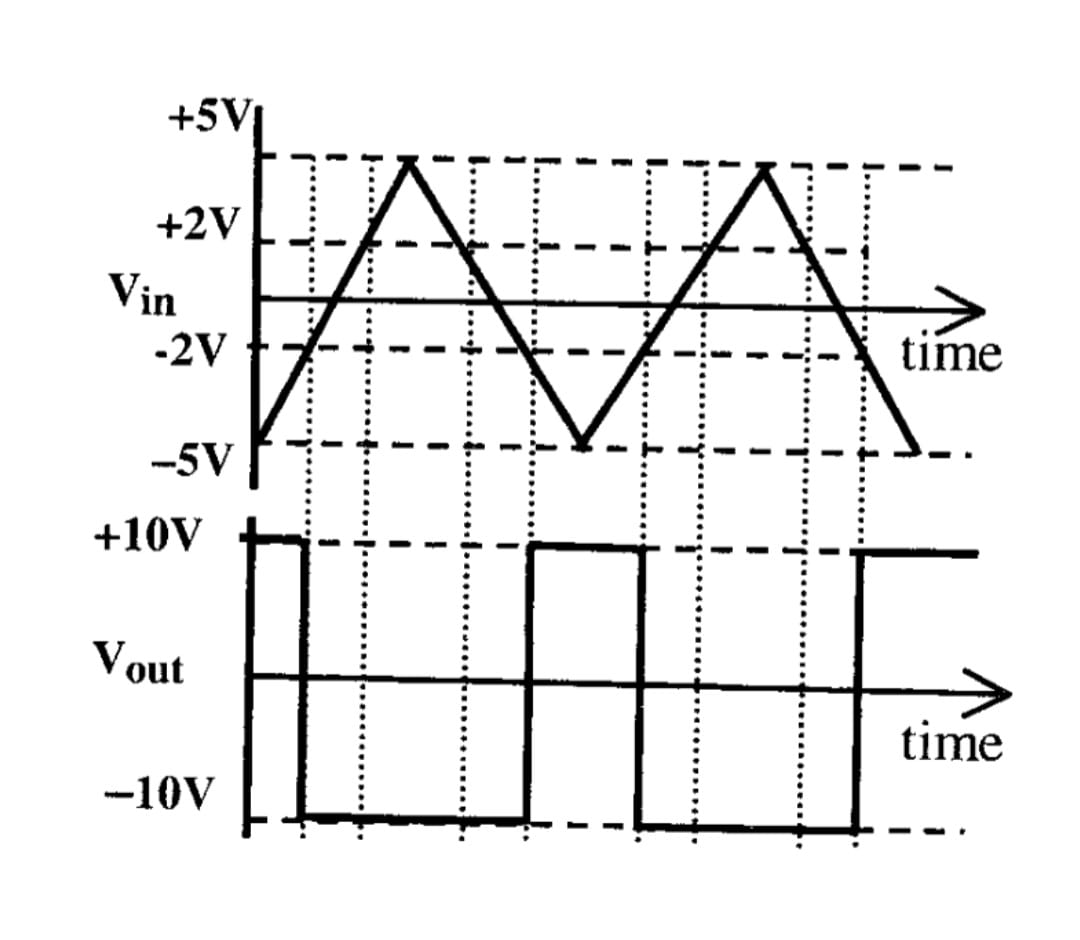
\includegraphics[width=0.25\textwidth]{fig11.jpeg} \hfill
\end{enumerate}
\end{multicols}


\newpage

\textbf{Common Data for Questions 48 and 49:} \\
Consider the function $f(z)=\frac{z\sin z}{(z-\pi)^2}.$ of a complex variable $z$,

\vspace{2em}

\item Which of the following statements is TRUE for the function $f(z)$?

\hfill{\brak{\text{GATE IN 2011}}}

\begin{enumerate}
    \item $f(z)$ is analytic everywhere in the complex plane
    \item $f(z)$ has a zero at $z=\pi$
    \item $f(z)$ has a pole of order $2$ at $z=\pi$
    \item $f(z)$ has a pole at $z=\pi$
\end{enumerate}


\item Consider a counterclockwise circular contour $|z|=1$ about the origin. The contour integral $\displaystyle\oint_{|z|=1} f(z)\,dz$ is

\hfill{\brak{\text{GATE IN 2011}}}

\begin{multicols}{4}
\begin{enumerate}
    \item $-i\pi$
    \item $0$
    \item $i\pi$
    \item $2i\pi$
\end{enumerate}
\end{multicols}


\textbf{Common Data for Questions 50 and 51:} \\

\vspace{2em}

The tight-binding energy dispersion relation for electrons in a one-dimensional array of atoms having lattice constant $a$ and total length $L$ is
\[
E = E_{0} - \beta - 2\gamma \cos(ka),
\]
where $E_{0}$, $\beta$ and $\gamma$ are constants and $k$ is the wave-vector. 

\item The density of states of electrons (including spin degeneracy) in the band is given by:

\hfill{\brak{\text{GATE IN 2011}}}

\begin{multicols}{2}
\begin{enumerate}
    \item $\dfrac{L}{\pi\, \hbar a \,\sin(ka)}$
    \item $\dfrac{L}{2\pi\, \gamma a \,\sin(ka)}$
    \item $\dfrac{L}{\pi a \,\cos(ka)}$
    \item $\dfrac{L}{2\pi a \,\cos(ka)}$
\end{enumerate}
\end{multicols}

\item The effective mass of electrons in the band is given by:

\hfill{\brak{\text{GATE IN 2011}}}

\begin{multicols}{2}
\begin{enumerate}
    \item $\dfrac{\hbar^{2}}{\gamma a^{2}\cos(ka)}$
    \item $\dfrac{\hbar^{2}}{2\gamma a^{2}\cos(ka)}$
    \item $\dfrac{\hbar^{2}}{\gamma a^{2}\sin(ka)}$
    \item $\dfrac{\hbar^{2}}{2\gamma a^{3}\sin(ka)}$
\end{enumerate}
\end{multicols}

\newpage

\textbf{Statement for Linked Answer Questions 52 and 53:} \\
In a one-dimensional harmonic oscillator, $\varphi_{0}$, $\varphi_{1}$, and $\varphi_{2}$ are respectively the ground, first, and second excited states. These three states are normalized and orthogonal to one another. Two states $\psi_{1}$ and $\psi_{2}$ are defined by:
\[
\psi_{1} = \varphi_{0} - 2\varphi_{1} + 3\varphi_{2}, \quad
\psi_{2} = \varphi_{0} - \varphi_{1} + \alpha \varphi_{2},
\]
where $\alpha$ is a constant.


\item The value of $\alpha$ for which $\psi_{2}$ is orthogonal to $\psi_{1}$ is:

\hfill{\brak{\text{GATE IN 2011}}}

\begin{multicols}{4}
\begin{enumerate}
\item $2$
\item $1$
\item $-1$
\item $-2$
\end{enumerate}
\end{multicols}

\item For the value of $\alpha$ determined above, the expectation value of energy of the oscillator in the state $\psi_{2}$ is:

\hfill{\brak{\text{GATE IN 2011}}}

\begin{multicols}{4}
\begin{enumerate}
\item $\pi \hbar \omega$
\item $\frac{3\hbar\omega}{2}$
\item $3\hbar\omega$
\item $\frac{9\hbar\omega}{2}$
\end{enumerate}
\end{multicols}


\textbf{Statement for Linked Answer Questions 54 and 55:} \\
A plane electromagnetic wave has the magnetic field:
\[
\vec{B}(x,y,z,t) = B_{0} \sin\left[\frac{k(x+y)}{\sqrt{2}} + \omega t\right] \, \hat{k},
\]
where $k$ is the wave number and $\hat{i}, \hat{j}, \hat{k}$ are the Cartesian unit vectors in $x$, $y$, and $z$ directions respectively.


\item The electric field $\vec{E}(x,y,z,t)$ corresponding to the above wave is:

\hfill{\brak{\text{GATE IN 2011}}}

\begin{multicols}{2}
\begin{enumerate}
\item $\dfrac{cB_{0}}{\sqrt{2}} \sin\left[\frac{k(x+y)}{\sqrt{2}} + \omega t\right](\hat{i} - \hat{j})$
\item $\dfrac{cB_{0}}{\sqrt{2}} \sin\left[\frac{k(x+y)}{\sqrt{2}} + \omega t\right](\hat{i} + \hat{j})$
\item $cB_{0} \sin\left[\frac{k(x+y)}{\sqrt{2}} + \omega t\right] \hat{i}$
\item $cB_{0} \sin\left[\frac{k(x+y)}{\sqrt{2}} + \omega t\right] \hat{j}$
\end{enumerate}
\end{multicols}

\item The average Pointing vector is:

\hfill{\brak{\text{GATE IN 2011}}}

\begin{multicols}{2}
\begin{enumerate}
\item $\dfrac{cB_{0}^{2}}{2\mu_{0}\sqrt{2}} (\hat{i} - \hat{j})$
\item $-\dfrac{cB_{0}^{2}}{2\mu_{0}\sqrt{2}} (\hat{i} - \hat{j})$
\item $\dfrac{cB_{0}^{2}}{2\mu_{0}\sqrt{2}} (\hat{i} + \hat{j})$
\item $-\dfrac{cB_{0}^{2}}{2\mu_{0}\sqrt{2}} (\hat{i} + \hat{j})$
\end{enumerate}
\end{multicols}

\newpage

\item Choose the most appropriate word from the options given below to complete the following sentence.\\
If you are trying to make a strong impression on your audience, you cannot do so by being understated, tentative or

\hfill{\brak{\text{GATE IN 2011}}}

\begin{multicols}{2}
\begin{enumerate}
    \item hyperbolic
    \item restrained
    \item argumentative
    \item indifferent
\end{enumerate}
\end{multicols}

\item Choose the most appropriate word(s) from the options given below to complete the following sentence.\\
I contemplated \rule{2cm}{0.15mm} Singapore for my vacation but decided against it.

\hfill{\brak{\text{GATE IN 2011}}}

\begin{multicols}{2}
\begin{enumerate}
    \item to visit
    \item having to visit
    \item visiting
    \item for a visit
\end{enumerate}
\end{multicols}

\item If $\log P = \frac{1}{2} \log Q = \frac{1}{3} \log R$, then which of the following options is TRUE?

\hfill{\brak{\text{GATE IN 2011}}}

\begin{multicols}{2}
\begin{enumerate}
    \item $P^{2} = Q^{3} \cdot R^{2}$
    \item $Q^{2} = PR$
    \item $Q^{2} = R^{3} \cdot P$
    \item $R = P^{2} \cdot Q^{2}$
\end{enumerate}
\end{multicols}

\item Which of the following options is the closest in meaning to the word below: \textbf{Inexplicable}

\hfill{\brak{\text{GATE IN 2011}}}

\begin{multicols}{2}
\begin{enumerate}
    \item Incomprehensible
    \item Indelible
    \item Inextricable
    \item Infallible
\end{enumerate}
\end{multicols}

\item Choose the word from the options given below that is most nearly opposite in meaning to the given word: \textbf{Amalgamate}

\hfill{\brak{\text{GATE IN 2011}}}

\begin{multicols}{2}
\begin{enumerate}
    \item merge
    \item split
    \item collect
    \item separate
\end{enumerate}
\end{multicols}

\item A transporter receives the same number of orders each day. Currently, he has some pending orders (backlog) to be shipped. If he uses 7 trucks, then at the end of the 4th day he can clear all the orders. Alternatively, if he uses only 3 trucks, then all the orders are cleared at the end of the 10th day. What is the minimum number of trucks required so that there will be no pending order at the end of the 5th day?

\hfill{\brak{\text{GATE IN 2011}}}

\begin{multicols}{2}
\begin{enumerate}
    \item 4
    \item 5
    \item 6
    \item 7
\end{enumerate}
\end{multicols}

\item The variable cost ($V$) of manufacturing a product varies according to the equation $V = 4q$ where $q$ is the quantity produced. The fixed cost ($F$) of production of the same product reduces according to the equation $F = \frac{100}{q}$. How many units should be produced to minimize the total cost $(V+F)$?

\hfill{\brak{\text{GATE IN 2011}}}
 
\begin{multicols}{2}
\begin{enumerate}
    \item 5
    \item 4
    \item 7
    \item 6
\end{enumerate}
\end{multicols}

\item P, Q, R and S are four types of dangerous microbes recently found in a human habitat. The area of each circle with its diameter printed in brackets represents the growth of a single microbe surviving human immunity system within 24 hours of entering the body. The danger to human beings varies proportionately with the toxicity, potency and growth attributed to a microbe shown in the figure below:

\begin{figure}[ht!]
    \centering
    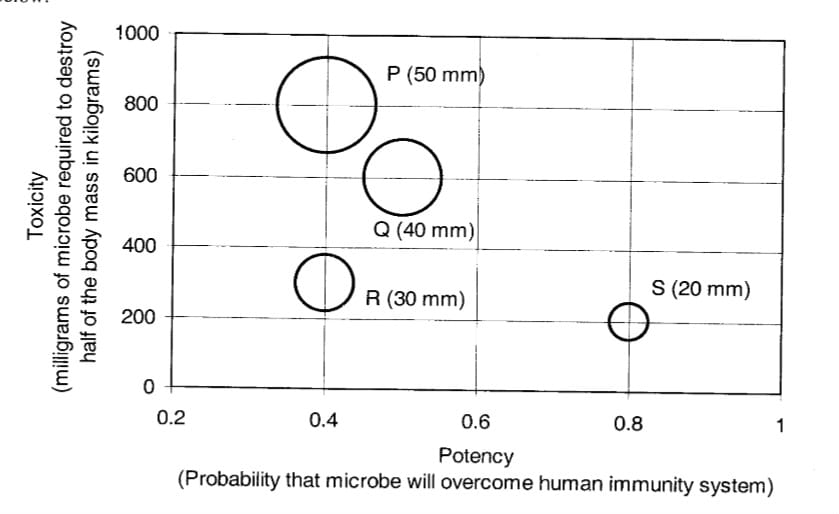
\includegraphics[width=0.75\textwidth]{fig12.jpeg}
    \caption{}
    \label{fig:fig12.jpeg}
\end{figure}

A pharmaceutical company is contemplating the development of a vaccine against the most dangerous microbe. Which microbe should the company target in its first attempt?

\hfill{\brak{\text{GATE IN 2011}}}

\begin{multicols}{4}
\begin{enumerate}
    \item P
    \item Q
    \item R
    \item S
\end{enumerate}
\end{multicols}

\item Few school curricula include a unit on how to deal with bereavement and grief, and yet all students at some point in their lives suffer from losses through death and parting.\\
Based on the above passage which topic would not be included in a unit on bereavement?

\hfill{\brak{\text{GATE IN 2011}}}


\begin{enumerate}
    \item how to write a letter of condolence
    \item what emotional stages are passed through in the healing process
    \item what the leading causes of death are
    \item how to give support to a grieving friend
\end{enumerate}


\item A container originally contains 10 litres of pure spirit. From this container 1 litre of spirit is replaced with 1 litre of water. Subsequently, 1 litre of the mixture is again replaced with 1 litre of water and this process is repeated one more time. How much spirit is now left in the container?

\hfill{\brak{\text{GATE IN 2011}}}

\begin{multicols}{4}
\begin{enumerate}
    \item 7.58 litres
    \item 7.84 litres
    \item 7 litres
    \item 7.29 litres
\end{enumerate}
\end{multicols}



\end{enumerate}

\vspace{2em}

\begin{center}
    \textbf{END OF THE QUESTION PAPER}
\end{center}

\end{document}
